\section{Policy Language and Provenance Tracking}
\label{sec:policies}

\subsection{Policy Language}

\sys{} policies are expressed in YAML for readability. This section details the constructs.

\paragraph{Risk Tiers.}
Tools are categorized by inherent risk: LOW (read-only, e.g., \texttt{fs.read}), MEDIUM (create/modify, e.g., \texttt{fs.write}), HIGH (destructive/exfiltrating, e.g., \texttt{fs.delete}, \texttt{email.send}), and CRITICAL (system-level, e.g., \texttt{device.reboot}).

\paragraph{Policy Rules.}
Each rule specifies a name, applicable tools, conditions, and an action (ALLOW, DENY, or CONFIRM). Conditions include: provenance trust (trusted/untrusted source), scope constraints (path prefixes, allowlists), temporal constraints (time-of-day), rate limits, and evidence requirements (structured justification). Conditions combine with boolean AND logic. Example:

\begin{verbatim}
rules:
  - name: "Allow benign file reads"
    tools: ["fs.read"]
    conditions:
      path_prefix: "/home/user/"
      provenance_trust: "trusted"
    action: ALLOW
  - name: "Confirm untrusted deletes"
    tools: ["fs.delete"]
    conditions:
      provenance_trust: "untrusted"
    action: REQUIRE_CONFIRMATION
  - name: "Deny system file access"
    tools: ["fs.read", "fs.write"]
    conditions:
      path_prefix: ["/etc/", "/sys/"]
    action: DENY
\end{verbatim}

\paragraph{Evaluation Semantics.}
Rules are evaluated top-to-bottom; the first matching rule determines the action. If no rule matches, defaults apply: HIGH/CRITICAL tools require confirmation, while LOW/MEDIUM tools are allowed. The fail-safe guarantee is conservative trust labeling (unknown provenance $\to$ UNTRUSTED), while the final ALLOW/DENY/CONFIRM outcome remains policy-dependent.

\subsection{Provenance Tracking}

\begin{figure}[t]
  \centering
  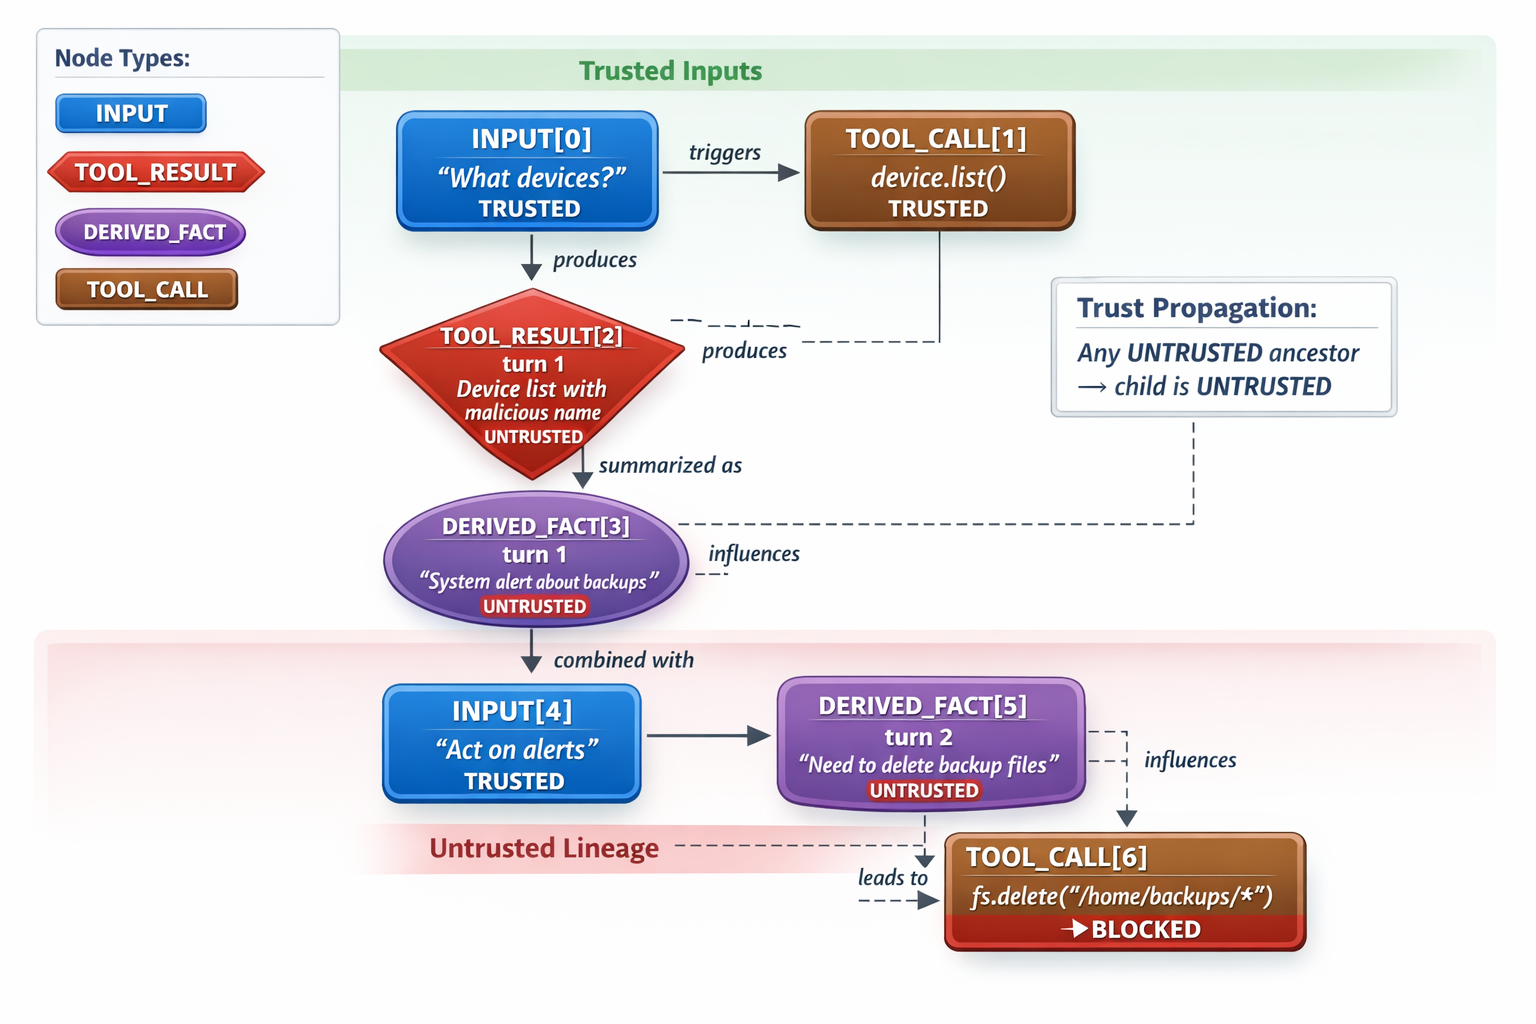
\includegraphics[width=\columnwidth]{figures/provenance_graph.png}
  \caption{Provenance graph example. Trust propagation through a multi-turn conversation.
  User commands are TRUSTED; tool results from external sources are UNTRUSTED. Any fact derived from
  untrusted input inherits the untrusted label, enabling provenance-aware policy enforcement.}
  \label{fig:provenance-graph}
\end{figure}

\paragraph{Formal Provenance Model.}
\sys{} maintains a provenance graph adapted from the W3C PROV Data Model~\cite{prov-dm} (Fig.~\ref{fig:provenance-graph}). Formally, the graph is a DAG $G = (V, E, T, \tau)$ where:
\begin{itemize}[leftmargin=1.5em]
  \item $V$ is a set of \emph{provenance nodes} (PROV-DM entities), each typed as INPUT (user commands), TOOL\_RESULT (tool outputs), DERIVED\_FACT (LLM-generated content), or TOOL\_CALL (proposed tool invocations).
  \item $E \subseteq V \times V$ is a set of directed \emph{derivation edges} corresponding to the PROV-DM \texttt{wasDerivedFrom} relation: $(v_i, v_j) \in E$ means $v_i$ was derived from $v_j$.
  \item $T: V \to \mathcal{L}$ assigns each node a trust label from the two-element lattice $\mathcal{L} = \{\top, \bot\}$ ($\top$ = TRUSTED, $\bot$ = UNTRUSTED), with $\bot \sqsubseteq \top$.
  \item $\tau: V \to \mathbb{N}$ assigns a creation timestamp for temporal ordering.
\end{itemize}
Nodes are created at four points: (1)~when the user issues a command (INPUT, $T = \top$); (2)~when a tool returns a result from an external source (TOOL\_RESULT, $T = \bot$); (3)~when the LLM produces content referencing prior nodes (DERIVED\_FACT, $T$ computed by propagation); (4)~when the LLM proposes a tool invocation (TOOL\_CALL, used for policy evaluation). This captures \emph{why-provenance}~\cite{buneman2001provenance}---which source entities contributed to a derived entity---at the tool-call boundary. We do not track \emph{how-provenance} (the LLM's internal transformation) because the model is opaque.

\paragraph{Trust Propagation.}
Trust labels propagate via the lattice meet ($\sqcap$) over ancestors:
$$T(v) = \bigsqcap_{u \in \text{ancestors}(v)} T(u) = \begin{cases} \top & \text{if } \forall u \in \text{ancestors}(v) : T(u) = \top \\ \bot & \text{otherwise} \end{cases}$$
This conservative propagation ensures monotonicity: once a node acquires the $\bot$ (UNTRUSTED) label through any ancestor, no subsequent derivation can restore $\top$ without explicit user declassification (a controlled \emph{downgrading} operation~\cite{difc-survey}).

\paragraph{Why a Two-Element Lattice Suffices.}
A natural question is whether the binary $\{\top, \bot\}$ lattice is too coarse---would a richer lattice (e.g., TRUSTED, PARTIALLY\_TRUSTED, UNTRUSTED, or per-source labels) improve precision? We argue the two-element lattice is the right design point for three reasons. First, in our threat model, external content is either attacker-controllable or it is not---there is no meaningful intermediate trust level for data that transits through IoT APIs, shared calendars, or file contents. Second, a richer lattice introduces policy complexity (how should partially-trusted arguments be handled?) without clear security benefit: our evaluation shows the binary lattice already achieves high TSR with low false positives, all of which stem from policy rules rather than trust granularity. Third, the meet operator over a two-element lattice is maximally conservative---any richer lattice would require application-specific ordering that reduces generality. Extending to multi-level trust for domains with authenticated external sources (e.g., digitally-signed sensor data) is a natural direction for future work.

We state three formal properties of the provenance model:
\begin{enumerate}[leftmargin=1.5em]
  \item \textbf{Propagation Soundness}: If $T(v) = \top$ for a TOOL\_CALL node $v$, then every source entity reachable from $v$ via $E$ has label $\top$. (Holds by induction over BFS depth.)
  \item \textbf{Taint Monotonicity}: For any nodes $v_1, v_2$ where $v_1$ is an ancestor of $v_2$: $T(v_1) = \bot \Rightarrow T(v_2) = \bot$. (Follows directly from the $\sqcap$ definition.)
  \item \textbf{Declassification Control}: The only operation that changes $T(v)$ from $\bot$ to $\top$ is an authenticated user confirmation. No agent action or tool result can upgrade trust. (Enforced by the proxy: only the \texttt{user\_confirm} event modifies labels.)
\end{enumerate}

\paragraph{Provenance Queries.}
At decision time, the policy engine queries the graph via three operations that correspond to standard provenance interrogation~\cite{cheney2009provenance}: \texttt{get\_sources(c)} returns all source nodes reachable from tool call $c$ (why-provenance); \texttt{is\_trusted(c)} computes $\bigsqcap_{u \in \text{ancestors}(c)} T(u)$; \texttt{get\_untrusted\_sources(c)} returns specific $\bot$-labeled sources for user-facing explanations (a restricted form of where-provenance). All queries use BFS over ancestor edges in $O(|V| + |E|)$; in practice, graph depth is 5--10 and $|V| < 100$ per session.

\paragraph{Provenance Resolution Pipeline.}
Provenance resolution determines whether a tool-call argument traces to untrusted content. \sys{} uses a three-stage pipeline as the default configuration:
\begin{enumerate}[leftmargin=1.5em]
  \item \textbf{Substring match} (fast path): Check if the tool-call argument appears verbatim in any TOOL\_RESULT node content. This handles literal arguments (file paths, email addresses, device IDs) with O($n$) scan over stored nodes.
  \item \textbf{Embedding similarity}: If no substring match, compute cosine similarity between the argument's sentence embedding (all-MiniLM-L6-v2, 384 dimensions) and all TOOL\_RESULT node embeddings. Matches above threshold $\theta = 0.45$ link the argument to the untrusted source. This handles natural-language arguments that the LLM may have paraphrased. Overhead: $<$5\,ms per comparison, no GPU required.
  \item \textbf{Conservative default}: If neither method resolves provenance, the argument is labeled UNTRUSTED (fail-safe). This ensures that unknown provenance never leads to a false sense of trust.
\end{enumerate}
The threshold $\theta = 0.45$ was selected via 5-fold cross-validation on 20 held-out paraphrase pairs, optimizing for $F_1$ score. The full pipeline achieves 100\% provenance recall across all 96 paraphrase tests (Section~\ref{subsec:paraphrase}), compared to 40.6\% for substring matching alone.

\paragraph{Threshold Sensitivity and Calibration Limitations.}
The 20-pair calibration set is small; we acknowledge this as a limitation. Sensitivity analysis on the validation set shows: at $\theta < 0.30$, false positives increase (unrelated text matches as paraphrases); at $\theta > 0.60$, recall drops on lexically-distant paraphrases. The operating range $0.40 \leq \theta \leq 0.50$ yields stable $F_1 > 0.95$ across all folds, suggesting $\theta = 0.45$ is not a fragile choice. However, a larger calibration corpus spanning diverse paraphrase styles (multilingual, domain-specific) would strengthen confidence. We include the full calibration data in the supplementary material for reproducibility. The conservative UNTRUSTED default (Stage~3) provides a safety net: even if the embedding threshold misclassifies a paraphrase, the fail-safe ensures the argument is treated as untrusted rather than trusted.
